\documentclass{article}
\usepackage[margin=1in]{geometry}
\usepackage{amsmath,amsfonts,amssymb}
\usepackage{listings}
\usepackage{color}
\usepackage{graphicx}
\usepackage{subfig}
\usepackage{blkarray}
\usepackage{multirow}
\usepackage{float}
\usepackage{caption}
\usepackage{subcaption}
\begin{document}
\begin{titlepage}
	\setlength{\parindent}{0pt}
	\large

\vspace*{-2cm}

\definecolor{dkgreen}{rgb}{0,0.6,0}
\definecolor{gray}{rgb}{0.5,0.5,0.5}
\definecolor{mauve}{rgb}{0.58,0,0.82}

\lstset{frame=tb,
  language=Python,
  aboveskip=3mm,
  belowskip=3mm,
  showstringspaces=false,
  columns=flexible,
  basicstyle={\small\ttfamily},
  numbers=none,
  numberstyle=\tiny\color{gray},
  keywordstyle=\color{blue},
  commentstyle=\color{dkgreen},
  stringstyle=\color{mauve},
  breaklines=true,
  breakatwhitespace=true,
  tabsize=3
}

University of Waterloo \par
CS 480 \par
\vspace{0.05cm}
r2knowle: 2023-10-22
\vspace{0.2cm}

{\huge Exercise \# 1 \par}
\hrule

\vspace{0.5cm}
\textbf{Q1)} Below is the code used to run the soft margin SVM, hard margin SVM and Logit:
\begin{lstlisting}
from sklearn import svm
from statsmodels.discrete.discrete_model import Logit
import sys
import pandas as pd

train_x = pd.read_csv("datasets/X_train_A.csv", header=None)
train_y = pd.read_csv("datasets/Y_train_A.csv", header=None)

logit = Logit(train_y, train_x).fit()

svm_soft = svm.SVC(C=1, kernel='linear')
svm_soft.fit(train_x, train_y)

svm_hard = svm.SVC(C=sys.maxsize, kernel='linear')
svm_hard.fit(train_x, train_y)


print(svm_soft.predict(train_x))
print(svm_hard.predict(train_x))
\end{lstlisting}
When running this code we get the following error for Logit:
\begin{verbatim}
  PerfectSeparationWarning: Perfect separation or prediction detected, parameter may 
    not be identified
\end{verbatim}
From the slides in the lectures we know that Logit try's to maximize the weights such that:
\[ \hat{w}= \text{arg}\text{min}\frac{1}{n} \sum_{i=1}^n l_w(x_i, y_i) \]
Now in order to optimize this we want to find where the gradient of the loss is 0. In other wards we need to find:
\[ \frac{1}{n} \sum_{i=1}^n \delta l_w(x_i, y_i) = 0\]
However since the data is perfectly separable, the loss will always be zero and so the derivative will never change. In other words we cant optimize as our MLE will be undetermined or infinite. To fix this we can introduce a misclassified point to avoid it being perfectly seperable. \\
The soft margin SVM will allow us to miss classify some points as the hyper plane used to separate the points can have some classification errors. On the other hand a hard margin SVM will always try to linearly separate the data so that theres no classification errors, in the event that this doesnt exist it wont return any parameters.
\newpage
\textbf{Q2)} We get that out of the 2000 elements, all 2000 of them are less then or equal to one. We got this by running the following code:
\begin{lstlisting}
rows = train_x.shape[0]
values = 0
for row in range(0, rows):
    current = train_x.iloc[row]
    sum = 0
    for val in range(0, len(current)):
        sum += current[val]*svm_soft.coef_[0][val]
    if (sum <= 1):
        values += 1
        
print(values)
\end{lstlisting}
Since all the data points can be classified this implies that the dataset can be linearly separable which makes the dataset seem to be in the form of: \\
\begin{center}
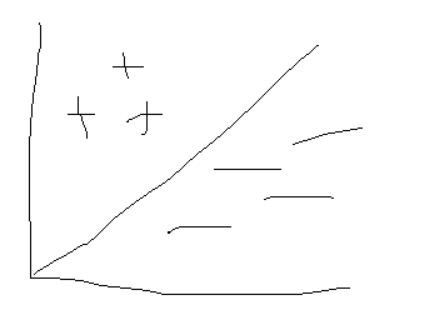
\includegraphics[width=0.5\textwidth]{g4.png}
\end{center}
The support vector for the soft margin SVM is:
\[ [1999,  1998] \]
In order to write the support vector as a linearly combinations of points we only need 2.\\\\
After running the second dataset, the hard margin SVM fails as the data is not linearlly separable. Our support vector is of size 192, and we got that from extracting it from the model. The accuracy on dataset B for the soft margin SVM we get:
\[ 97.15\%\]
\end{titlepage}
\end{document}